\section{Arquitectura l�gica}

La arquitectura l�gica definida para la herramienta corresponde al patr�n Modelo-Vista-Controlador~\cite{Syromiatnikov2014}. La elecci�n de este patr�n se debe a que permite la separaci�n de la l�gica de negocio y la vista presentada al usuario logrando de esta manera una aplicaci�n altamente mantenible y con una mejor escalabilidad. El diagrama que representa la arquitectura usada para el desarrollo se puede ver en la Figura~\ref{fig:arquitectura_logica}.  

\begin{figure}[H]
    \centering
    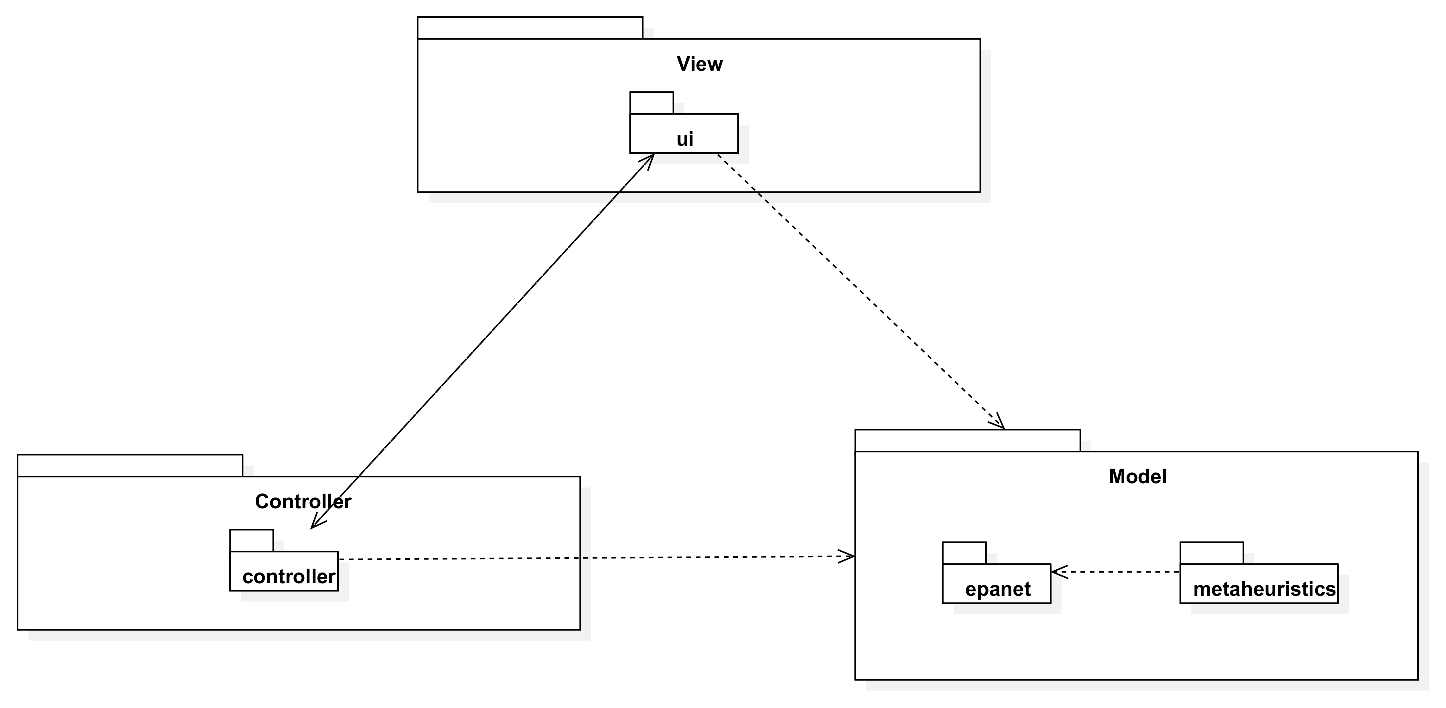
\includegraphics[width=\textwidth]{Capitulo2/assets/arquitectura_logica.eps}
    \caption{Arquitectura l�gica.}
    \label{fig:arquitectura_logica}
\end{figure}

En el diagrama presentado en la Figura \ref{fig:arquitectura_logica} se presencia la divisi�n de la aplicaci�n en tres capas. La capa Vista se encarga de la interacci�n con el usuario y de la interfaz de usuario. La capa Controlador se encarga de responder a los eventos de los usuarios y solicitar informaci�n a la capa de modelo. La capa Modelo contiene la informaci�n y la l�gica fundamental de la aplicaci�n en un formato adecuado para interactuar con las dem�s capas. Esta �ltima capa, tambi�n se encarga de la ejecuci�n de los algoritmos y la interacci�n con la librer�a nativa EpanetToolkit.

La capa Modelo se divide principalmente en dos componentes. Estos componentes son:

\paragraph{Componente Metaheur�sticas (\textit{Metaheuristics}):}
Modulo que contiene los algoritmos, operadores, los tipos de soluci�n permitidos y los problemas que ser�n abarcados durante el desarrollo del proyecto. 

\paragraph{Componente Hidr�ulico (EPANET):}
El m�dulo hidr�ulico posee las clases necesarias para cargar los archivos de red (inp) y generar una representaci�n de ellos a trav�s de una serie de clases. Este m�dulo tambi�n se encarga de guardar la representaci�n de una red ya modificada en un archivo inp para que pueda ser usado por el programa EPANET. Las simulaciones hidr�ulicas ser�n realizadas usando la librer�a epajava. Esta librer�a realiza las llamadas nativas a la EpanetToolkit. La librer�a epajava puede ser descargada en el repositorio de git ubicado en https://github.com/jhawanet/epajava .
